\documentclass{article}

% Top margin, right margin, left margin, bottom margin, footnote skip
\usepackage[utf8]{inputenc}
\usepackage{biblatex}
\addbibresource{./references.bib}
% linktocpage shall be added to snippets.
\usepackage{hyperref,theoremref}
\hypersetup{
	colorlinks, 
	linkcolor={red!40!black}, 
	citecolor={blue!50!black},
	urlcolor={blue!80!black},
	linktocpage % Link table of content to the page instead of the title
}

\usepackage{blindtext}
\usepackage{enumitem}
\usepackage{algorithm}
\usepackage{algpseudocode}
\usepackage{titlesec}
\usepackage{amsthm}
\usepackage{thmtools}
\usepackage{amsmath}
\usepackage{amssymb}
\usepackage{graphicx}
\usepackage{titlesec}
\usepackage{xcolor}
\usepackage{multicol}
\usepackage{breqn}
\usepackage{hyperref}
\usepackage{import}
\usepackage{libertinus}           % Load the Libertinus font
\usepackage{mathbbol}
\usepackage{bm}
\usepackage{mathrsfs}

\usepackage{chngcntr}
\counterwithin*{equation}{section}
\renewcommand{\theequation}{\thesection.\arabic{equation}}

\usepackage{tikz}
\usepackage{tikz-cd}
\usetikzlibrary{arrows.meta, positioning, calc, arrows, quotes, math, angles}
% \usepackage{calrsfs}


\newtheorem{theorem}{Theorem}[section]
\newtheorem{corollary}[theorem]{Corollary}
\newtheorem{proposition}[theorem]{Propostion}
\theoremstyle{definition}
\newtheorem{lemma}[theorem]{Lemma}
\newtheorem{definition}[theorem]{Definition}
\newtheorem{problem}{Problem}


\theoremstyle{remark}
\newtheorem{remark}[theorem]{Remark}
\newtheorem{example}[theorem]{Exampli Gratia}
% Proof Environments
\newcommand{\thm}[2]{\begin{theorem}[#1]{}#2\end{theorem}}

% \renewenvironment{proof}{{\bfseries\emph{Demonstratio.}}}{\qed}





\renewcommand{\L}{\mathcal{L}}
\newcommand{\C}{\mathcal{C}}

\renewcommand{\H}{\mathcal{H}}


\newcommand{\Z}{\mathbb{Z}}
\newcommand{\D}{\mathbb{D}}
\newcommand{\sq}{\frac{1}{\sqrt{2}}}

\newcommand{\id}{\text{id}}

\newcommand{\im}{\text{Im}}

\newcommand{\ket}[1]{|#1\rangle}
\newcommand{\bra}[1]{\langle#1|}

\newcommand{\kp}{\ket{\psi}}

\newcommand{\lde}{\text{lde}}


\renewcommand{\emph}{\textbf}
\renewcommand{\Re}{\text{Re}}

\usepackage{tikzit}



\title{A Survey of Approximation of Single Qubit Unitaries with Clifford and T Gates}
\author{Candidate Number: 1099144} 
\date{\today}

\begin{document}

\maketitle

\abstract{
	This survey is written for the assessment of the course	Introduction to Quantum Information at Oxford. 
	We reviewe the basic concepts of quantum computation and discuss in detail the universality of Clifford and T gates. 
	We summarise the Mastumoto-Amano normal form, which is a unique representation of single qubit unitaries over Clifford and T gates with minimal T-count. We also discuss the Ross-Selinger algorithm for approximating $z$-rotations using Clifford and T gates.
}

\tableofcontents

\section{Brief Introduction to Quantum Computation}

Computations, regardless of how it is performed, at its most fundamental level is a physical process. 
Human perform computations in our mind by the biochemical process that took place in the brain, classical computer by transmitting electronic signals in the circuit boards, and \textit{quantum computers} by manipulating and measuring  the states of quantum mechanical objects.

The following postulates of quantum mechanics is key to our discussions
\begin{enumerate}[label={\textbf{Postulate} \arabic*}]
	\item the simplest quantum state is \textit{qubit}, which is described by unit vector in $\mathbb{C}^2$;
	\item composition of $n$-qubit state is described by unit vector in $(\mathbb{C}^2)^{\otimes n} \cong \mathbb{C}^{2^n}$;
	\item states evolved by unitary\footnote{$U$ is unitary if $U^\dagger U = I$} operations.
	\item quantum measurement is governed by the Born rule.
\end{enumerate}

We will dicuss the first three postulates here, while leaving the discussion of Born rule to section \ref{sec:measurement}.

Let $\ket{1} = \begin{pmatrix}1 \\ 0\end{pmatrix}$ and $\ket{0} = \begin{pmatrix}0 \\ 1\end{pmatrix}$ be the standard orthonormal basis of $\mathbb{C}^2$.
Any one qubit state $\ket{\psi}$, therefore, can be described as 
$$
\ket{\psi} = a\ket{0} + b\ket{1}, \quad a, b \in \mathbb{C}, |a|^2 + |b|^2 = 1
$$

The following unitary operators are called Pauli operators, which will be important for later discussions and are presented here as examples of unitaries operations.
\begin{equation}\label{eq:pauli}
	X = \begin{pmatrix}
0 & 1\\
1 & 0
\end{pmatrix}, \quad Y = \begin{pmatrix}0 & -i\\
i & 0
\end{pmatrix}, \quad Z = \begin{pmatrix}1 & 0\\
0 & -1
\end{pmatrix}
\end{equation}

It is worth discussing why states evolve according to unitary matrices.
The time evolution of a closed quantum state $\ket{\psi}$ is described by the \textit{Schrödinger equation}

\begin{equation}\label{schrodinger}
	i \hslash \frac{d \ket{\psi}}{d t} = H \ket{\psi}
\end{equation}
If $H$ is a time independent Hamiltonian, the solution \eqref{schrodinger} is 
$$
\ket{\psi(t)} = e^{\frac{-iH t}{\hslash}} \ket{\psi(0)}
$$
where $\ket{\psi(0)}$ is the initial state of the system.
Standard results from linear algebra show that for Hermitian $H$, $e^{\frac{-i H t}{\hslash}}$ is indeed unitary for any real $t$.

The existence of qubit systems in nature has been demonstrated by the famous Stern-Gerlach experiment \cite{Sakurai_Napolitano_2020}. 
Various physical realisations of quantum computers have been proposed, such as those based on ion traps \cite{steane1997ion}, optical photon \cite{gardiner2004quantum}, and nuclear magnetic resonance \cite{nmr} among others.

In this article we will regard qubit and its unitary evolution as our fundamental quantum mechanical system and describe the theories of unitary operation.

\subsection{Single Qubit Operation}

The Bloch sphere representation of a qubit is very helpful for our discussion.
Any qubit $\ket{\psi}$ can be written $\ket{\psi} = a \ket{0} + b \ket{1}$ for some $a , b \in \mathbb{C}$ such that $|a|^2 + |b|^2 = 1$.
If we write $|a| = \cos \frac{\theta}{2}$ and $|b| = \sin \frac{\theta}{2}$, then for some phase factors $e^{i \alpha}$ and $e^{i \beta}$, we have
$$
\ket{\psi} = e^{i \beta} \left(\cos \frac{\theta}{2} \ket{0} + e^{i \alpha} \sin \frac{\theta}{2} \ket{1}\right),
$$

We can represent $\ket{\psi}$ as a point on the unit sphere, where $\theta$ and $\alpha$ denote the polar and azimuthal angles. 
This is called a Bloch sphere.

\begin{figure}[htbp]
	\centering
	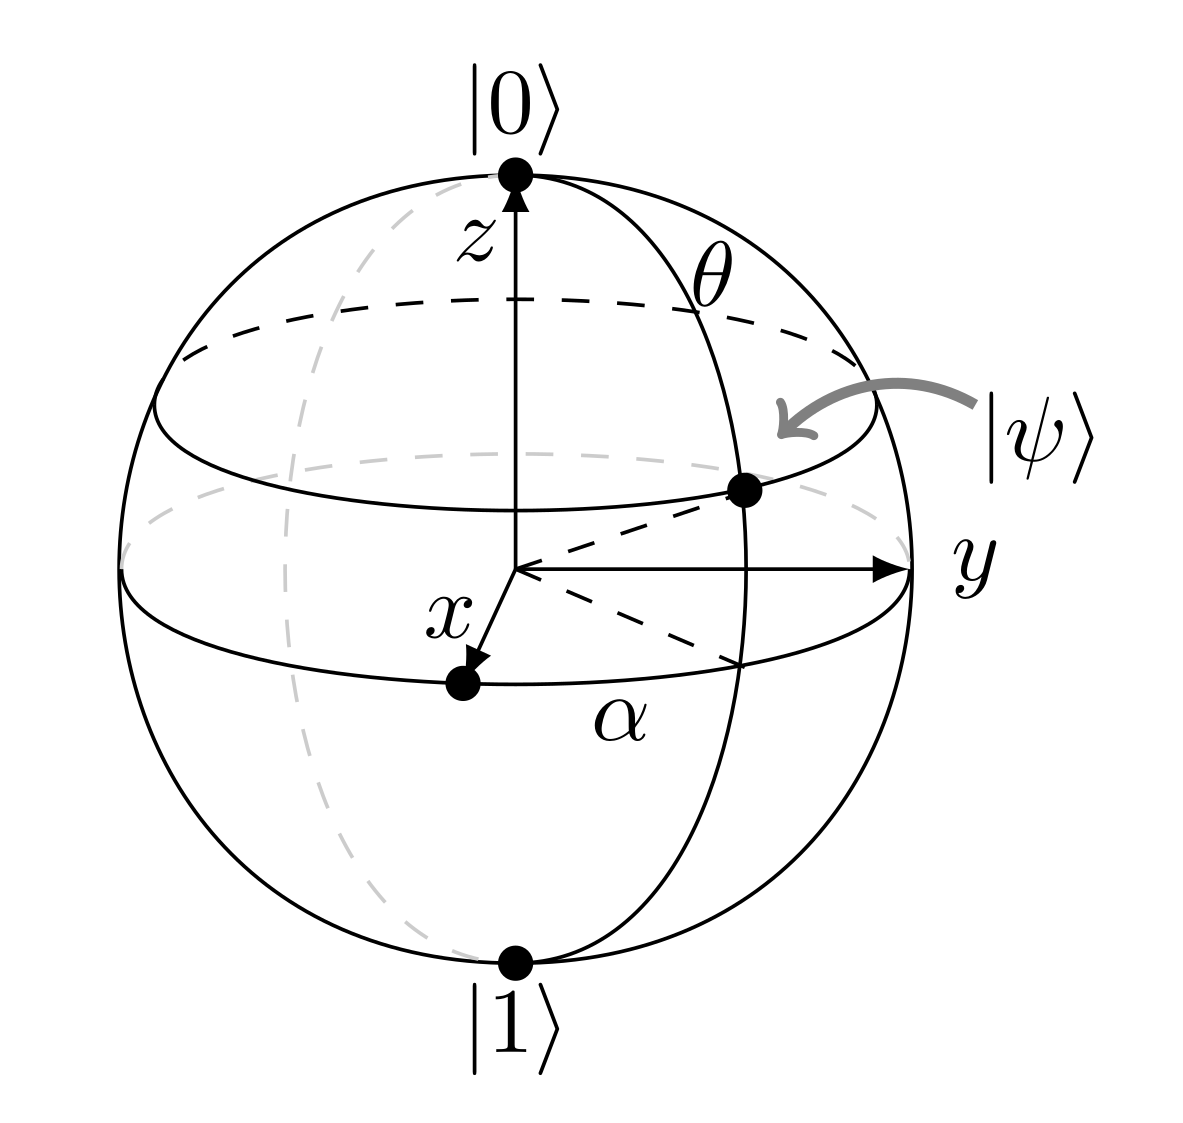
\includegraphics[width=0.5\textwidth]{./figures/bloch.png}
	\caption{Bloch Sphere}
	\label{fig:Bloch Sphere}
\end{figure}

The action of Pauli $Z$ from \eqref{eq:pauli} on the block sphere is.
\begin{dmath*}
	Z \ket{\psi} = Z \ket{\psi} 
	= e^{i \beta} \left(\cos \frac{\theta}{2} \ket{0} - e^{i \alpha} \sin \frac{\theta}{2} \ket{1}\right)
	= e^{i \beta} \left(\cos \frac{\theta}{2} \ket{0} + e^{i \alpha + \pi} \sin \frac{\theta}{2} \ket{1}\right)
\end{dmath*}
It transforms $(\theta, \alpha)$ to $(\theta, \alpha + \pi)$, which is rotation by $\pi$ on $z$ axis.
By similar arguments, we can show Pauli $X, Y$ in \eqref{eq:pauli} correspond to the rotations of $\pi$ along the $x, y$ axis.
It turns out that unitary operations on a single qubit are precisely the rotations on Bloch sphere.

\begin{theorem}[Unitaries on Bloch Sphere]\label{th:unitary-bloch}
	The actions of single-qubit unitary matrices is equivalent to rotation (represented by $SO(3)$) in the Bloch sphere.
\end{theorem}
This theorem is excercise 4.6 from \cite{Nielsen_Chuang_2010}.


\subsection{Measurement}\label{sec:measurement}

Our discussion of measurement is breif and only for the sake of completeness. 
For more details see chapter 2.2 and 4.4 of \cite{Nielsen_Chuang_2010}.

Recall that a positive semidefinite projector is a Hermitian matrix $M$ such that $M^2 = M$ and $\bra{\psi} M \ket{\psi} \geq 0$ for any $\ket{\psi}$. 
Using spectral theorem, we can show that each positive semidefinite projector $M$ can be written as
$$M = \sum_{i} c_i\ket{v_{i}} \bra{v_{i}}, \quad c_i \in \{0, 1\}$$
where $\ket{v_{i}}$ is a set of orthonormal basis of $\mathbb{C}^2$.
That is, the eigenvalues of a positive semidefinite projector are either 0 or 1. 

Let $\mathcal{M} = \{M_1, M_2, \cdots, M_n\}$ be a set of positive semidefinite projectors $V \rightarrow V$ such that $\sum_{i=1}^n M_i = I$. 
Each of $M_i$ is called an observable of the measurement $\mathcal{M}$.
Given a state $\kp$, the probability of obtaining the outcome $i$ is $\bra{\psi} M_i \ket{\psi}$, and the post-measurement state is $\frac{M_i \ket{\psi}}{\sqrt{\bra{\psi} M_i \ket{\psi}}}$.

This principle of obtaining probabilistic outcomes from measurement is called the Born rule.

From Born rule, we see $\kp$ and $e^{i\pi \theta} \kp$ are indistinguishable for any $\theta \in \mathbb{R}$, since 
$$
\bra{\psi} M_i \ket{\psi} = \bra{\psi} e^{-i\pi \theta} M_i e^{i\pi \theta} \ket{\psi}
$$


\subsection{Univeral Gates}

In the effort to build quantum computers one task is especially important: to find some small sets of unitary matrices that can effectively simulate any unitary operations.
These unitary matrices are called universal gates.

Let us first concentrate on the single-qubit unitary operations.
There are infinitely many single qubit unitary operations, making it impossible to exactly synthesize any arbitrary operation with a finite set of gates. 
\footnote{On classical computers, it is well known that NAND gate alone is sufficient to implement any Boolean function \cite{sheffer1913set}.}
Therefore, we relax our goal to find a finite set of gates that can approximate any single qubit unitary operation to arbitrary precision in the sense defined below. 

\begin{definition}[Error of approximation]
	If $U$ is the unitary operation we wish to implement while $V$ is the actual implementation in practice. 
	The \emph{error} of approximation is defined as  
	\begin{equation}
		E(U, V) = \max_{\ket{\psi}} \frac{\| (U - V) \ket{\psi} \|}{\| \ket{\psi} \|}.
	\end{equation}
\end{definition}

This definition of error has two important properties which fits our intuitions for errors. 
\begin{enumerate}
	\item Let $\ket{\psi}$ be our initial state. If $E(U, V)$ is small, the probability of obtaining different measurement outcome from $U \kp$ and $V \kp$ is small;
	\item accumulated error satisfies triangular inequality, that is 
		$$
			E(U_1 U_2, V_1, V_2) \leq E(U_1, V_1) + E(U_2, V_2)
		$$
\end{enumerate}

Their proofs are presented in the appendix \ref{sec:error}.

With the proper definition for error, we can settle the definition of univera;l gate.
\begin{definition}[Universal Gate]
A set of quantum gates is called \emph{universal} if any unitary operation can be aproximated with arbitraily small error by a finite sequence of gates from the set.
\end{definition}

\subsubsection{Universality of Hadamard and T Gates and CNOT}

An important set of universal gate which we discuss in detail here is Hadamard + T gate. 
Where Hadamard gate $H$ and T gate $T$ are defined as
\begin{equation*}
		H = \frac{1}{\sqrt{2}} \begin{pmatrix}
		1 & 1\\
		1 & -1
		\end{pmatrix}, \quad T = \begin{pmatrix}
		1 & 0\\
		0 & e^{i\pi/4}
		\end{pmatrix}.
\end{equation*}

\begin{remark}
	Note that both of $T$ and $H$ are unitary, and $T^4 = Z$ and $HZH = X$.
\end{remark}

\begin{theorem}
	The set $\{H, T\}$ is a universal gate set for single qubit unitary operations.
\end{theorem}

\begin{proof}
	We can write
	$$
	T = \cos \frac{\pi}{8} I - i \sin \frac{\pi}{8} Z, \quad H = \frac{1}{\sqrt{2}} (X + Z).
	$$
	where $X, Z$ are the Pauli X and Z operators, respectively. 
	Calculation shows that 
	$$
	THTH = \cos^2\frac{\pi}{8} I - i \sin \frac{\pi}{8} \left( \cos \frac{\pi}{8} (X + Z) + \sin \frac{\pi}{8} Y \right),
	$$
	This is rotation along the axis $(\cos\frac{\pi}{8}, \sin\frac{\pi}{8}, \cos\frac{\pi}{8})$ through an angle $\theta$ defined by $\cos \frac{\theta}{2} = \cos^2 \frac{\pi}{8}$.
	We can show that $\theta$ is a irrational multiple of $\pi$\footnote{See \cite{boykin1999} and section 4.5.3 of \cite{Nielsen_Chuang_2010}. }.
	Therefore repeated applications of $THTH$ can approximate any rotation along the axis $(\cos\frac{\pi}{8}, \sin\frac{\pi}{8}, \cos\frac{\pi}{8})$ to arbitrary precision.

	By the same calculation we can show that $HTHT$ is a rotation along the axis $(\cos\frac{\pi}{8}, -\sin\frac{\pi}{8}, \cos\frac{\pi}{8})$ through the same angle $\theta$. 
	Repeated applications of $HTHT$ can approximate any rotation along the axis $(\cos\frac{\pi}{8}, -\sin\frac{\pi}{8}, \cos\frac{\pi}{8})$ to arbitrary precision.

	As shown in the appendix, any single qubit unitary $U$ can be represented as 
	$$
	U = R_{\hat{n}}(\alpha) R_{\hat{m}}(\beta) R_{\hat{n}}(\gamma),
	$$
	where $\hat{n}$ and $\hat{m}$ are two non-parallel axes, and $R_{\hat{n}}(\alpha)$ denotes the rotation along axis $\hat{n}$ through angle $\alpha$.

	Previous paragraphs shows that for any $\epsilon > 0$, $H$ and $T$ can be used to approximate generate $V_1, V_2, V_3$ such that $E(R_{\hat{n}}(\alpha), V_1) < \epsilon$, $E(R_{\hat{m}}(\beta), V_2) < \epsilon$ and $E(R_{\hat{n}}(\gamma), V_3) < \epsilon$.
	Applying proposition \ref{prop:cumulation-of-error} we see $E(U, V_1 V_2 V_3) < 3 \epsilon$, proving the universality of $H$ and $T$.
\end{proof}

So $H$ and $T$ gates can approximate any single qubit unitary operation.
The surprising fact is that by adding one more gate, CNOT, they can be used to approximate any unitary operation on any number of qubits. 

\begin{theorem}
	Single qubit gates together with CNOT gate is a universal gate set for quantum computation.
\end{theorem}

\begin{proof}
	The detailed proof can be found here \cite{barenco1995elementary}.
	The gist of the proof is two parts 
	\begin{enumerate}
		\item any multi-qubit unitary operations can be decomposed into two-body unitary operations via Gaussian elimination. \footnote{By two-body unitary operation we mean a unitary operation that acts non-trivially on only a 2-dimensional subspace.} 
		\item any two-body unitary operation can be implemented by CNOT and single qubit gates.
	\end{enumerate}
\end{proof}



\section{Exact Synthesis of Single Qubit Clifford+T Circuits}

In this section, we present results from Kliuchnikov et al \cite{exact-clifford+t} on an algorithm for the exact synthesis of single-qubit unitaries over the Clifford + T gate set, when it is possible.

The key insight is the following theorem, which relates the set of unitaries that can be implemented by Clifford+T circuits with the ring $\Z\left[\frac{1}{\sqrt{2}}, i\right]$.
\begin{theorem}\label{unitary-iff-clifford+t}
	Denote $\mathcal{CT}(2)$ as the set of all $2 \times 2$ unitary matrices that can be exactly implemented by a single qubit Clifford+T circuit. 
	Then $U \in \mathcal{CT}(2)$ if and only if $U \in U(\Z\left[\frac{1}{\sqrt{2}}, i\right])$, which is to say it is an unitary matrix with entries in $\Z\left[\frac{1}{\sqrt{2}}, i\right]$.

	In such a case, moreover, it can be written in the following form
	\begin{equation}\label{clifford+t-form}
	\begin{pmatrix}
		a & b^\dagger \omega^k \\ 
		b & a^\dagger \omega^k \\	
	\end{pmatrix}
	\end{equation}
	where $a, b \in \Z\left[\frac{1}{\sqrt{2}}, i\right]$, $\omega = e^{\pi i/4}$ and $k$ is an integer, and $\dagger$ denotes the complex conjugate.
\end{theorem}


\begin{remark}\label{rk:first-column-matters}
Notice that 
$$
\begin{pmatrix}
		a & b^\dagger \omega^k \\ 
		b & a^\dagger \omega^k \\	
	\end{pmatrix} T^n 
	= \begin{pmatrix}
		a & b^\dagger \omega^{k+n} \\ 
		b & a^\dagger \omega^{k+n} \\	
\end{pmatrix}
$$
This means we only need to regard the first column of any unitary matrix in finding a Clifford+T circuit that implements it.
As for any $U, V \in \mathcal{CT}(2)$ with the same first column, we have $U = VT^n$ for some integer $n$.
\end{remark}


\begin{definition}[Least Denominator Exponent]\label{def:lde}
	The least denominator exponent of a vector or matrix $u$ with entries in the ring $\Z[\sq, i]$, denoted as $\lde(u)$, is the smallest non-negative integer $k$ such that $\sqrt{2}^k u$ has entries in $\Z[\omega]$.
\end{definition}

By theorem \ref{unitary-iff-clifford+t}, all $U$ that can be implemented by Clifford+T circuits have entries in $\Z[\sq, i]$, so they have a well-defined least denominator exponent.

The least denominator exponent is a measure of how far a unitary matrix is from being implementable by Clifford gates alone, as Clifford gates have entries in $\Z[i]$ and thus have least denominator exponent $0$.
We can use the following theorem to reduce the least denominator exponent of a unitary matrix by applying $H$ and $T$ gates.

\begin{theorem}\label{lde-reduction}
	Let $U \in \mathcal{CT}(2)$,
	let $\text{lde-tl}(U)$ denote $\lde(|z|^2),$ where $z$ is its top left entry.
	Assuming $\text{lde-tl}(U) \geq 4$
	Then there exists $k \in \{0, -1, -2, -3\}$ such that $\text{lde-tl}(H T^k U) = \text{ldt-tl}(U) - 1$.
\end{theorem}

There are only finitely many unit vectors $v$ such that $\lde(|v|^2) \leq 4$.
As the column of a unitary matrix $U \in \mathcal{CT}(2)$ is a unit vector, we can reduce $\text{ldt-tl}(U)$ to a small enough number, after which we can find a Clifford+T circuit that implements it by brute-force search.

We list the exact steps of the algorithm \ref{exact-synthesis-algorithm} for clarity.

\begin{algorithm}[ht]\label{exact-synthesis-algorithm}
	\caption{Exact Synthesis of Single Qubit Unitaries over Clifford+T}
	\hspace*{\algorithmicindent} \textbf{Input:} $U \in \mathcal{CT}(2)$ \\
\hspace*{\algorithmicindent} \textbf{Output:} a sequence of $H$ and $T$ gates that implements $U$
\begin{algorithmic}[1]
	\State $M \gets U, R \gets I$ \Comment{$M$ is temporary matrix, $R$ stores the result}
	\While{$\text{lde-tl}(M) \geq 4$} \label{while-loop-exact-synthesis}
	\State find $k \in \{0, -1, -2, -3\}$ such that $\text{lde-tl}(H T^k M) = \text{lde-tl}(M) - 1$ \Comment{Guaranteed by theorem \ref{lde-reduction}}
\State $M \gets H T^k M$ 
\State $R \gets R T^{-k} H$
\EndWhile 
\State Using brute force to find a sequence of $H$ and $T$ gates that implements $M$. Label this sequence as $M_s$\Comment{There are only finitely many options with $\lde \leq 2$}
\State $R \gets M_s \cdot R$
\State \textbf{return} $R$
\end{algorithmic}
\end{algorithm}

The major work of the algorithm is the while loop in line \ref{while-loop-exact-synthesis}.
After each iteration, the result is appended with $TH, SH, $ or $TSH$. 
So the run time of the algorithm is linear in the number of gates in the output circuit.
Combining with Mastumoto-Amano normal form discussed in the next section, it can be shown that the T-count of this algorithm is optimal.

The case of multi-qubit unitaries that can be generated by Clifford+T circuits is more complicated. 
Kliuchnikov et al hypothesize that any unitary matrix that can be implemented by a Clifford+T circuit has entries in $\Z\left[\frac{1}{\sqrt{2}}, i\right]$.

\section{Mastumoto-Amano Normal Form}

Single-qubit Clifford + T circuits can be written in the form of 
$$
	C_n T C_{n-1} T \cdots C_1 T C_0
$$
where each $C_n$ is some Clifford circuit.

Matsumoto and Amano \cite{matsumoto} showed that every single qubit Clifford + T circuit can be written in the following more restrictive form. 
$$
	W_n T W_{n-1} T \cdots W_1 T C
$$
where $W_n \in \{I, H, SH\}$, $W_i \in \{H, SH\}$ and $C$ is some Clifford circuit.
This is called the \textit{Matsumoto-Amano normal form}.

The importance of the Mastumoto-Amano normal form is summarised in the following theorem.

\begin{theorem}\label{thm:matsumoto-amano}
	T-count of the normal form is optimal.
\end{theorem}

We can, in addition, show that 
\begin{lemma}
\begin{enumerate}
		\item Every single qubit Clifford + T circuit can be written uniquely in the Matsumoto-Amano normal form. 
		\item A linear time algorithm exists to compute the normal form of a given single qubit Clifford + T circuit, with respect to the number of gates of the input.
	\end{enumerate}
\end{lemma}

\subsection{Existence}

We shall prove Theorem \ref{thm:matsumoto-amano} by the following lemmas.
Recall we have the following elementary quantum gates:
$$
H = \frac{1}{\sqrt{2}}\begin{pmatrix}
1 & 1 \\
1 & -1
\end{pmatrix}, \quad S = \begin{pmatrix}
1 & 0 \\
0 & i
\end{pmatrix}, \quad T = \begin{pmatrix}
1 & 0 \\
0 & e^{i\pi/4}
\end{pmatrix}, \quad \omega = e^{i\pi/4} I
$$

In all of the following lemmas, let $\mathcal{C}$ denote the one-qubit Clifford group generated by $H, S,$ and $\omega$. 
Let $\mathcal{L}$ denote the its subgroup generated by $S, X, $ and $\omega$, where $X = HS^2H$ is the Pauli X gate. 
Let $\C ' =  \C \backslash \L$.
Let $\mathcal{H} = \{I, S, SH\}$ and $\mathcal{H}' = \{H, SH\}$.

\begin{lemma}
	$\L$ has three left cosets in $\C$, namely $\L, H\L,$ and $SH\L$. 
	So $\C = \H \L$ and $\C' = \H' \L$.
\end{lemma}

\begin{proof}
	It is well known that the order of $\C$ is $192 = 64 \cdot 3$ \cite{mastel2025cliffordtheorynqubitclifford}. 
	The group $\L = (S, X, \omega)$ has the following structure
	$$
	XS = S^3 \omega^2 X, \omega S = S \omega, \omega X = X \omega, S^4 = I, X^2 = I, \omega^8 = I
	$$
	so all element of $L$ can be written as $\omega^i S^j X^k$ for some power $i, j, k$.
	As $\omega$ has order $8$, $S$ has order $4$ and $X$ has order $2$, $|L| = 4 \cdot 2 \cdot 8 = 64$.

	This means $L$ has three left cosets.
	Now, a simple calculation shows that $H\L$ and $SH\L$ are the other two left cosets, so $\C = \H \L$.
	$\C'$ is the complement of $\L$ in $\C$, so $\C' = \H' \L$.
\end{proof} 

\begin{lemma}
	$\L \H ' \subseteq \H ' \L$
\end{lemma}

\begin{proof}
	Since $S \in \L$, we have $\L\H' = \L S \cup \L SH \subset \L H$, which is non-trivial right coset of $\L'$.
	The non-trivial right coset must be a subset of the $\C' = \C \backslash \L = \H'\L$.
\end{proof}

\begin{lemma}
	$\L T = T \L$.
\end{lemma}

\begin{proof}
	$T$ commutes with generators of $\L$ in the following way
	$$
	ST = TS, XT = T XS \omega^{-1}, \omega T = T \omega 
	$$
	Thus for all $l \in \L$ we have another $l' \in \L$ s.t. $lT = Tl$, which means $\L T = T \L$.	
\end{proof}

\begin{lemma}\label{TLT=L}
	$T\L T = \L$
\end{lemma}

\begin{proof}
	Notice that $T\L T = TT \L = S\L = \L$, as $S \in \L$.	
\end{proof}

We are now ready to prove the existence of the Matsumoto-Amano normal form.

\begin{proof}[Proof: Uniqueness of Matsumoto-Amano normal form]
	By definition, Clifford + T circuits can be written as 
	$$M = C_n T C_{n-1} T \cdots C_1 T C_0.$$
	If any of the intermediate $C_i \in \L$ for $i\in \{1, 2, \cdots, n-1\}$, use $\ref{TLT=L}$ to reduce $TC_iT$ into another Clifford, which will merge the its adjacent $C_{i+1}, C_{i-1}$. 
	Doing so reduces $T$ counts by $2$.
	
	After reducing all intermediate $C_i$, our gates will be in the set 
	\begin{dmath}
	M 
	= \C T \C' T \cdots T \C' T \C
	=  \H \L T \H' \L T \cdots T \H' \L T \H \L
	\end{dmath}
	We can move all the $\L$ to the right of $\H'$ and $T$, this gives 
	$$
	M = \H T \H' T \cdots T \H' T \H \L
	$$
	which is the desired Matsumoto-Amano normal form.
\end{proof}

This proof is constructive, giving us a linear-time algorithm to reduce any Clifford + T circuit into the Matsumoto-Amano normal form, which is the second part of Theorem \ref{thm:matsumoto-amano}.

\begin{proof}
	Since $\C$ is a finite group, we may assume computation in $\C$ takes constant time using a hash table.
	As $\L$ is a subgroup of $\C$, identifying whether an element is in $\L$ also takes constant time.
	
	Starting with a given input in the form
	$$M = C_n T C_{n-1} T \cdots C_1 T C_0.$$
	we can check from left to right whether $C_i \in \L$ for $i\in \{1, 2, \cdots, n-1\}$. 
	If $C_i$ is in $\L$, replace $C_{i+1} T C_i T C_{i-1}$ with an element in $\L$. 
	At each step, we are moving rightwards by $2$ gates, so this process takes at most $O(n)$ time.

	After reducing all intermediate $C_i$, we can move all $\L$ to the right of $\H'$ and $T$ with the same process.
\end{proof}

\subsection{Optimality of T-count}

The aim of this section is to show the following theorem.

\begin{theorem}\label{thm:matsumoto-amano-uniqueness}
	Two Matsumoto-Amano normal forms represent the same unitary if and only if they are identical as circuits. 
	That is, they can be written down in the exact same way.
\end{theorem}

Assuming the correctness of theorem \ref{thm:matsumoto-amano-uniqueness}, we can show that the $T$-count of the Matsumoto-Amano normal form is minimal.

\begin{corollary}
	The number of $T$ gates in the Matsumoto-Amano normal form is minimal among all Clifford + T circuits representing the same unitary.
\end{corollary}

\begin{proof}
	Let $M$ be a Clifford + $T$ unitary with the minimal number of $T$ gates in its circuit representation. 
	Such a minimal representation exists by Zorn's lemma.

	We can reduce $M$ into its Matsumoto-Amano normal form $M'$ by the procedure described in the proof of the existence. 
	In that procedure, the number of $T$ gates may only decrease, so $M'$ will have the same number of $T$ gates as $M$.

	By uniqueness, all representations of $M$ can be reduced to the same normal form.
	This concludes the proof.
\end{proof}

The proof of \autoref{thm:matsumoto-amano-uniqueness} requires more sophisticated analysis on the structure of $\C$ and $\L$, which we will achieve in the following paragraphs using more tools in algebra.

As we have shown in  \autoref{sec:bloch-sphere}, all one-qubit unitaries, up to an insignificant global phase, can be represented as a rotation on the Bloch sphere.
As rotations in 3 dimensions are represented by $SO(3)$, we can represent each one-qubit unitary as an element in $SO(3)$, which is called the \textit{Bloch sphere representation} of the unitary.

\begin{definition}[Bloch Sphere Representation]
	Let $U SU(2)$, denote $\hat{U} \in SO(3)$ as the rotation on the Bloch sphere induced by $H$.
\end{definition}

For example, the Bloch sphere representation of $H$, $S$, and $T$ are:
\begin{equation}\label{eq:bloch-representation}
\hat{H} = \begin{pmatrix}
0 & 0 & 1 \\
0 & -1 & 0 \\
1 & 0 & 0
\end{pmatrix},  
\hat{S} = \begin{pmatrix}
0 & -1 & 0 \\
1 & 0 & 0 \\
0 & 0 & 1
\end{pmatrix},  
\hat{T} = \frac{1}{\sqrt{2}}\begin{pmatrix}
1 & -1 & 0 \\
1 & 1 & 0 \\
0 & 0 & \sqrt{2} \\
\end{pmatrix}
\end{equation}

\begin{remark}\label{remark:clifford-so3}
	Let $\hat{\C}$ denote the Bloch sphere representation of Clifford group, which is generated by $\hat{H}$ and $\hat{S}$.
	$\hat{H}$ is the linear transformation that permutes the $x, y, z$ axis to $z, -y, x$, and $\hat{S}$ permutes the $x, y, z$ axis to $-y, x, z$.
	Thus, all elements of  $\hat{\C}$ must be some permutation of the $x, y, z$ axis to $\pm x, \pm y, \pm z$.

	Let us use a temporary notation $(a, b, c)$ to denote the linear map that sends $x, y, z$ to $a, b, c$ respectively.

	Note 
	\begin{align*}
		\hat{H} &= (z, -y, x) \\
		\hat{S} \hat{H} &= (z, x, y)\\ 
		\hat{S}  &= (y, -x, z) \\
		\hat{S}^3 &= (-y, x, z)
	\end{align*}

	Both of $\hat{H}$ and $\hat{S}$ are odd permutations, which also brings one negative sign. 
	Ignoring the signs, we $\hat{S} \hat{H}$ and $\hat{S}$ are exactly the generators of the symmetric group $S_3$. 
	Combining these two observations, we see $\hat{C}$ consists of odd permutations of $x, y, z$ with an odd number of negative signs and even permutations of $x, y, z$ with an even number of negative signs.

	It turns out this is the only rule that needs to be satisfied for a linear map to be in $\hat{\C}$.
	This is because $\hat{S}$ swaps the first two axes while negating the second, and $\hat{S}^3$ swaps the first two axes while negating the first.
	Paired with $\hat{S}\hat{T}$, they can generate any permutation of two axes while negating either one of them.

	This means $\hat{\C}$ consists of $3! \cdot 8 / 2 = 24$ elements, which are exactly the elements of $SO(3)$ with entries only in $\pm 1$.
\end{remark}

Remark \ref{remark:clifford-so3} states that all Cliffords have Bloch sphere representation with entries $\pm 1$. 
Equation \ref{eq:bloch-representation} shows that $T$ has Bloch sphere representation with entries that are the sum and product of integers and $\sq$. This is exactly the ring of numbers $\Z[\sq]$.

Since Clifford + T circuits are generated by Clifford and $T$, we have the following proposition.

\begin{proposition}
	The Bloch sphere representation of any Clifford + T circuit is an a matrix in $SO(3, \mathbb{Z}[\frac{1}{\sqrt{2}}])$.
\end{proposition}

We define a map $q: SO(3, \Z[\sq]) \rightarrow Mat_{3, 3}(\Z / 2\Z)$ in the following way. 
For any $u \in SO(3, \Z[\sq])$, 
\begin{enumerate}
	\item Find the smallest $k$ such that $\left(\sq\right)^k u$ has entries in $\Z[\sqrt{2}]$.
	\item each entry of $\left(\sq\right)^k u$ can be written as $a + b\sqrt{2}$ for some integers $a, b$, we define the corresponding entry of $q(u)$ to be $a \mod 2$.
\end{enumerate}

The number $k$ is the \textit{least denominator exponent} of $u$.
We call $p(u)$ the \textit{parity form} of $u$.

Define an equivalence relationship $\sim$ on $SO(3, \Z[\sq])$ by $u \sim v$ if and only if $u $ and $v$ differ by a permutation of columns.

We have the following important lemma.

\begin{lemma}
	Let $M$ be the Bloch sphere representation of a Matsumoto-Amano normal form with least denominator exponent $k$.
	Then exactly one of the following holds:
	\begin{enumerate}
		\item $k = 0$, and $M$ is Clifford. 
		\item $k > 0$, and $q(M) \sim \begin{pmatrix}
1 & 1 & 0 \\ 
1 & 1 & 0 \\ 
0 & 0 & 0
\end{pmatrix}$ if the first gate of the normal form is $T$
		\item $k > 0$, and $q(M) \sim \begin{pmatrix}
0 & 0 & 0 \\ 
1 & 1 & 0 \\ 
1 & 1 & 0
\end{pmatrix}$ if the first gate of the normal form is $HT$
		\item $k > 0$, and $q(M) \sim \begin{pmatrix}
1 & 1 & 0 \\ 
0 & 0 & 0 \\ 
1 & 1 & 0
\end{pmatrix}$ if the first gate of the normal form is $SHT$
	\end{enumerate}
\end{lemma}

\begin{proof}
	Any Matsumoto-Amano normal form can be written as some Clifford left multiplied by some sequence of $HT$ and $SHT$, which terminates with an optional $T$.

	Elements of the Clifford group have a parity form of identity. 
	Direct computation shows that, when left multiplied by $T$, $HT$, or $SHT$, the parity form changes as illustrated by the scheme below, where $k++$ denotes the increment of the least denominator exponent by $1$.
	From which it is clear that the parity form of a normal form is completely determined by the first gate of the normal form.
\ctikzfig{ma-form}

\end{proof}

We are now ready to prove the uniqueness of the Matsumoto-Amano normal form.

\begin{proof}[Proof: Uniqueness of Matsumoto-Amano normal form]
	Let $M$ and $N$ be two Matsumoto-Amano normal of the same unitary map.
	Without loss of generality, let $T$ gate counts of $M$ be smaller than or equal to those of $N$.

	Since $M$ and $N$ represent the same unitary, they must have the same parity form of Bloch sphere representation. This means the starting gate of $M$ and $N$ must be the same, which is either $T$, $HT$, or $SHT$.
	We can then cancel the first gate of $M$ and $N$, and repeat the
	process until we have cancelled all $T$ gates of $M$, leaving us with a Clifford circuit with parity form of identity.
	At this moment, the parity form of $N$ must also be identity, so $N$ is also left with a Clifford circuit equal to that of $M$.
\end{proof}


\section{Approximation of Z-rotation Using Clifford+T}

\subsection{Overview of the Algorithm}

Building on the exact synthesis algorithm of Kliuchnikov et al. \cite{exact-clifford+t}, Ross and Selinger \cite{ross} proposed an efficient algorithm to use Clifford + $T$ gates to approximate single qubit $Z$-rotation in the following form 

$$
	R_z(\theta) = \begin{pmatrix}
		e^{-i\theta/2} & 0 \\
		0 & e^{i\theta/2} \\
	\end{pmatrix}.
$$

They showed that for all $\epsilon$, there exists a Clifford + $T$ circuit $U$ in the form of 
\begin{equation}\label{ross-form}
U = \begin{pmatrix}
	a & -b^\dagger \\ 
	b & a^\dagger
\end{pmatrix}
\end{equation}
such that $\|R_z (\theta) - U \| < \epsilon$.
By the results of Kliuchnikov et al., $a \in \Z[\sq, i]$. 
The insight of Ross and Selinger is that to find such $a, b \in \mathbb{C}$ (or show no such exists) with $\lde(a) = n$ is equivalent to solving the solving the following two problems:
\begin{enumerate}
	\item To find a possible value for $a$ is equivalent to enumerate a certain finite set in $\mathbb{R}^2$
	\item To find the corresponding $b$ is equivalent to solve a the Diophantine equation in $aa^\dagger + bb^\dagger = 1$.
\end{enumerate}
Both the enumeration of and solving the Diophantine equation takes polynomial time in $n$.
The algorithm starts with $n = 0$ and keep increasing $n$ until it finds a solution.
By an number-theoretical argument, they shows that the expected time this algorithm terminates is polynomial in $\log(1/\epsilon)$, and the resulting circuit has $T$-count at most $3 \log_2(1/\epsilon) + O(\log(\log(1/\epsilon)))$.

The detailed steps are shown in the following section.

\subsection{Details of the Algorithm}

\subsubsection{Two-dimensional Grid Enumeration}

Let us first consider the field $\Z[\omega]$, where $\omega = e^{\pi i/4}$.
We have the following equality
\begin{align*}
	\omega^4 &= -1 \\ 
	\omega^5 &= -\omega = \omega^{3 \dagger} \\
	\omega^6 &= -\omega^2 = \omega^{2 \dagger} \\ 
	\omega^7 &= -\omega^3 = \omega^{\dagger} \\
\end{align*}
There fore $\Z[\omega]$ is the free $\Z$-module generated by $1, \omega, \omega^2, \omega^3$.
Write $u \in \Z[\omega]$ as $u = a \omega^3 + b \omega^2 + c \omega + d$ for some $a, b, c, d \in \Z$.
Use the fact that $\omega = \frac{1}{\sqrt{2}} (1 + i)$, we have
\begin{align*}
	u &= (d + \frac{c-a}{2} \sqrt{2}) +  i (b + \frac{c+a}{2} \sqrt{2}) \\
\end{align*}
Since $c-a$ and $c+a$ have the same parity (they must both be even or both be odd), it follows that 
$$
u = \alpha + \beta \omega
$$
where $\alpha \in \Z[\sqrt{2}, i]$ and $\beta = 0, 1$.
This is summarised in the following lemma. 
\begin{lemma}\label{z-omega-form}
	Every element in $\Z[\omega]$ can be written as $\alpha$ or $\alpha + \omega$, where $\alpha \in \Z[\sqrt{2}, i]$.
\end{lemma}

Write $u \in \Z[\omega]$ as $u = a + \sqrt{2} b$, where $a, b \in \Z[i]$.
We define $u^{\bullet} = a - \sqrt{2}b$. That is, $(-)^{\bullet}$ is the unique ring automorphism of $\Z[\omega]$ that sends $\sqrt{2}$ to $-\sqrt{2}$ and fixes $i$.

We are now ready to describe Grid, the central idea of the enumeration algorithm.

\begin{definition}[Grid]
	Let $B$ be a subset of $\mathbb{C}$. The \emph{grid} of $B$ is the set of all $u \in \Z[\omega]$ such that $u^{\bullet} \in B$.
\end{definition}

Since there is a canonical isomorphism between $\mathbb{C}$ and $\mathbb{R}^2$ by identifying $x + iy$ with $(x, y)$, we can also regard the grid of $B$ as a subset of $\mathbb{R}^2$.
By adopting the convention in \cite{ross}, when describing two-dimensional grid problem, we will not distinguish between $\mathbb{C}$ and $\mathbb{R}^2$ and write $A, B$ as subsets of $\mathbb{R}^2$.

Using lemma \ref{z-omega-form}, we have the following innocuous looking lemma

\begin{lemma}[Discrete Grid]\label{discrete-grid}
	Let $U = \{(a + \sqrt{2} b, c + \sqrt{2} d)\}$ be subset of $\Z[\omega]$ where $a, b$ have the same sign, while $c, d$ have the same sign.
	Then $U$ is a discrete subset of $\mathbb{R}^2$, that is, for every bounded subset $A \subset \mathbb{R}^2$, the set $ U \cap A$ is finite.
\end{lemma}

\begin{proof}
	Using lemma \ref{z-omega-form}, any element in $\Z[\omega]$ can be written as $\alpha$ or $\alpha + \omega$, where $\alpha \in \Z[\sqrt{2} ,i]$.

	Let us first consider the case when $u = \alpha \in U$. 
	It can be written as $u = (a + b \sqrt{2}, c + d \sqrt{2})$ (where we use the canonical isomorphism to denote $\mathcal{C}$ as an element in $\mathbb{R}^2$).
	Since $u$ is in a bounded region, we may assume $|a + b\sqrt{2} | < \beta$ for some $\beta > 0$. Since $a$ and $b$, it is evident that there are only finitely many choices for $a$ and $b$.
	The same argument applies to $c$ and $d$. 

	The other case is exactly the same
\end{proof}

\begin{definition}[Two-dimensional Grid Problem]
	Let $A, B$ be subsets of $\mathbb{C}$.
	The two-dimensional grid problem for $A$ and $B$ is to find all $u \in \Z[\omega]$ such that $u \in A$ and $u^{\bullet} \in B$.
\end{definition}


An immediate observation is the following lemma. 

\begin{lemma}\label{grid-solution}
	If $B$ is a bounded convex and closed subset of $\mathbb{R}^2$ with non-empty interior and $A$ some bounded subset.
	There there exists only finitely many $u$ such that $u \in A$ and $u^{\bullet} \in B$.
\end{lemma}

\begin{proof}
	Let us try to find all $u$ such that $u \in A$ and $u^{\bullet} \in B$.

	Write $u^{\bullet} = (a + \sqrt{2} b, c + \sqrt{2} d)$. 
	Let us consider $a + \sqrt{2}b$ first. 

	There are two cases: $a, b$ have the same sign or they have different signs. 
	$u^\bullet \subset B$ and $B$ is bounded, by lemma \ref{discrete-grid} there exists only finitely many $a + \sqrt{2} b$ such that $a, b$ have the same sign and $a + \sqrt{2}b$ is in the bounded region.
	If it is in the second case, we have $u = (a - \sqrt{2} b , c - \sqrt{2}d)$. As $a, b$ are of different signs, $a, -b$ will have the same sign. Since $u \in A$ where $A$ is bounded, apply lemma \ref{discrete-grid} again, we have only finitely many choices for $a - \sqrt{2} b$.  

	The argument the the $y$ direction is the same, which completes the proof.
\end{proof}

An demonstration of the grid problem for $u \in [-5, 5] \times [-5, 5]$ and $u^\bullet [-1, 1] \times [-1, 1]$ is presented in figure \ref{fig:Demonstration of grid problem}.

\begin{figure}[htbp]
	\centering
	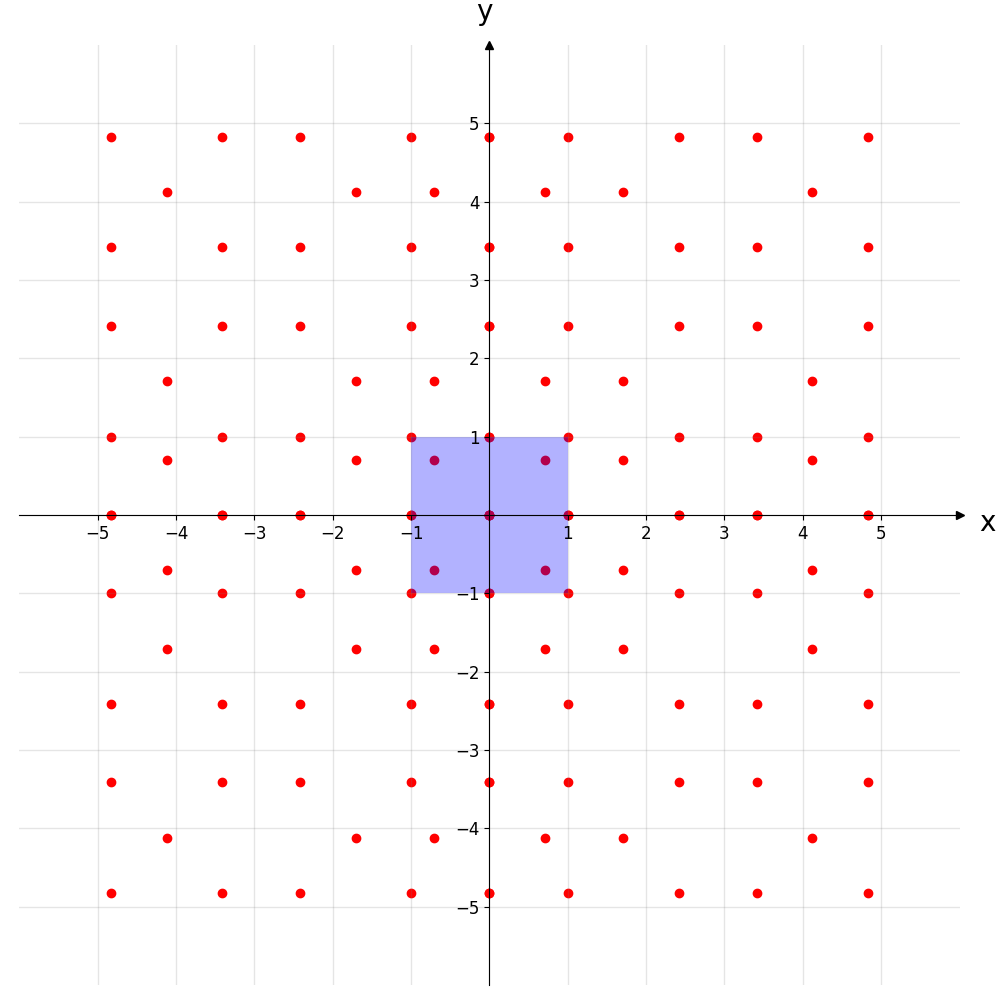
\includegraphics[width=0.6\textwidth]{./python/discrete-set.png}
	\caption{Solution to the Grid problem $u \in [-5, 5] \times [-5, 5]$ and $u^\bullet [-1, 1] \times [-1, 1]$.}
	\label{fig:Demonstration of grid problem}
\end{figure}

So for we have focused on the case when $u \in \Z[\omega]$, where the least denominator exponent of $u$ is $0$. (We used the same definition for least denominator exponent as in definition \ref{def:lde}.)
When the least denominator exponent of $u$ is some finite $n$, we can write $u = \frac{1}{\sqrt{2}^n} u'$, where $u' \in \Z[\omega]$. 
It is clear that the finiteness condition which we derived in lemma \ref{grid-solution} still holds for $u'$, so all of our arguments above can be applied to $u'$ with only minor modification.

In theorem \ref{grid-solution}, we have produced a finite set which contains all the solutions to the grid problem.
With some regularity constraints, we may assume that we can check whether a given $u$ is in the required set efficiently. \footnote{
	The details of the regularity constraints is complicated but are not too important for our discussion. Check \cite{ross} section 5.2, 5.3, 5.4 for more details.
}

This leads to central result of this section.

\begin{corollary}\label{grid-algorithm}
	For $u \in \Z[\sq, i]$ with finite least denominator exponent.
	Given a bounded convex and closed subset $B$ of $\mathbb{R}^2$ with non-empty interior and some bounded subset $A$, there is an efficient algorithm thatfinds all $u$ such that $u \in A$ and $u^{\bullet} \in B$.
\end{corollary}

From the results of \cite{exact-clifford+t}, we know that any single-qubit unitary that can be implemented by Clifford + $T$ gates must be in the form of 
\begin{equation}\label{clifford+t-form-1}
\begin{pmatrix}
	a & -b^\dagger \omega^l \\ 
	b & a^\dagger \omega^l \\
\end{pmatrix}
\end{equation}
where $a, b \in \Z[\sq, i]$, $\omega = e^{\frac{\pi}{4}}$ and $l$ is an integer. 

When approximating $R_z(\theta)$, however, we can show that $l = 0$.

\begin{lemma}
	Let $U$ be a single-qubit unitary generated by Clifford + $T$ gates. If $\|R_z{\theta} - U\| \leq |1 - e^{\frac{\pi}{8}}|$, then U must be in the form 
	\begin{equation}\label{clifford+t-form-nophase}
	\begin{pmatrix}
		a & -b^\dagger \\ 
		b & a^\dagger 
	\end{pmatrix}
	\end{equation}
	For some $a, b \in \Z[\sq, i]$.
\end{lemma}

\begin{proof}
	
\end{proof}

\subsubsection{Solving the Diophantine Equation}


\section{Conclusion}

In this report, we touched on one of the central problems in quantum computation: how to implement a given unitary operation using a finite set of gates, and how to do it efficiently. 
This is called the quantum compilation problem.

We have shown that the Clifford + T gate is a universal gate set.
Works by Kliuchnikov et al \cite{exact-clifford+t} proved the necessary and sufficient condition for a single qubit unitary to be exactly implementable by Clifford + T gates, and provided an efficient algorithm for finding such a circuit when it exists.
Matsumoto and Amano \cite{matsumoto} showed that any Clifford + T circuit can be transformed into a unique normal form with minimal T-count. 
This is particularly important as T gates are more expensive to implement than Clifford gates in fault-tolerant quantum computation.
Finally, we have also presented the Ross-Selinger algorithm for approximating $z$-rotations using Clifford and T gates, which is asymptotically optimal in terms of T-count.



\appendix 
\section{Quantifying Error of Unitary Operations}\label{sec:error}

\begin{remark}[Soundness of Definition of Error]
	Let $\ket{\psi}$ be the initial state of the system, which is evolved according to unitary $U$ or $V$, and then measured via POVM measurement $M$. 
	Let $P_U$ and $P_V$ denote the probability of obtaining the corresponding measurement outcome when the operator $U$ or $V$ are performed, respectively. 

	Then 
	$$
	|P_U - P_V| = | \bra{\psi} U^\dagger M U \ket{\psi} - \bra{\psi} V^\dagger M V \ket{\psi} |
	$$
	Let $\ket{\Delta} := (U - V)\ket{\psi}$, we have 
	\begin{align*}
		|P_U - P_V| 
		& = | \bra{\psi} U^\dagger M \ket{\Delta} + \bra{\Delta} M V \ket{\psi} | & \\
		&\leq | \bra{\psi} U^\dagger M \ket{\Delta} | + |\bra{\Delta} M V \ket{\psi} | &\\
		& \leq \| \ket{M^\dagger U \psi} \| \cdot \| \ket{\Delta} \| + \| \ket{M V \psi} \| \cdot \| \ket{\Delta} \|  & \text{(by Cauchy-Schwarz)}\\ 
		& \leq 2 \| \ket{\Delta} \| &  \| \ket{M^\dagger U \psi}\| \leq 1\\
		& = 2 E(U, V) &
	\end{align*}

	This means if $E(U, V)$ is small, the probability of obtaining a different measurement outcome is also small, which is exactly what we expect for the definition of error.
\end{remark}

\begin{proposition}[Cumulation of Error]\label{prop:cumulation-of-error}
	If we have a sequence of unitary operations $U_1, U_2, \cdots, U_n$ and their approximations $V_1, V_2, \cdots, V_n$ with error $E(U_i, V_i)$, then 
	$$
	E(U_1 U_2 \cdots U_n, V_1 V_2 \cdots V_n) \leq \sum_{i=1}^n E(U_i, V_i).
	$$
\end{proposition}

\begin{proof}
	Let us first consider $E(U_1U_2, V_1V_2)$
	By definition
\begin{align*}
	E(U_1U_2, V_1V_2) 
	& = \max_{\|\ket{\psi}\| = 1} \| (U_1 U_2 - V_1 V_2) \ket{\psi} \|&\\
	& = \max_{\|\ket{\psi}\| = 1} \| (U_1 U_2 - U_1 V_2 + U_1 V_2 - V_1 V_2) \ket{\psi} \| &\\
	& \leq \max_{\|\ket{\psi}\| = 1} \| \| (U_1 U_2 - U_1 V_2) \ket{\psi} \| + \| (U_1 V_2 - V_1 V_2) \ket{\psi} \| & \\
	& = E(U_2, V_2) + E(U_1, V_1) &
\end{align*}
The general case will follow from induction.
\end{proof}

The definition of error is echoes the definition of matrix 2-norm.

\begin{definition}[Matrix 2-norm]
	The matrix 2-norm of a matrix $M$ is defined as 
	$$
	\| M \| = \max_{\ket{\psi}} \frac{\| M \ket{\psi} \|}{\| \ket{\psi} \|}.
	$$
\end{definition}

\begin{proposition}[Computation of 2-Norm]
	Assuming $M$ is normal\footnote{A matrix $M$ is normal if $M M^\dagger = M^\dagger M$.}, 
	Then
	$$
	\| M \| = \max_{\ket{\psi}} \frac{\| M \ket{\psi} \|}{\| \ket{\psi} \|} = ||\lambda_{\max}|,
	$$
	Where $\lambda_{\max}$ is the eigenvalue of $U - V$ with the largest modulus.
\end{proposition}

\begin{proof}
	This is the standard result about matrix norm. 

	Since $M$ is normal by spectral theorem $M$ can be decompose into $\lambda_1\ket{u_1}\bra{u_1} + \lambda_2 \ket{u_2} \bra{u_2}$, where $\lambda_1, \lambda_2$ are its eigenvalues and $\ket{u_1}, \ket{u_2}$ are its orthogonal eigenvectors.

	Therefore any vector $\alpha$ can be written as $\alpha = a \ket{u_1} + b \ket{u_2}$ for some $a, b \in \mathbb{C}$, and we have

	\begin{align*}
		\frac{\|M \ket{\alpha}^2 \|}{\| \ket{\alpha}\|^2} 
				 &= \frac{\|M (a \ket{u_1} + b \ket{u_2})\|^2}{|a|^2 + |b|^2} 
				 &\\ 
				 & = \frac{\|a \lambda_1 \ket{u_1} + b \lambda_2 \ket{u_2}\|^2}{|a|^2 + |b|^2} 
				 &\\ 
				 & \leq \frac{ |a|^2 |\lambda_1|^2 + |b|^2 |\lambda_2|^2}{|a|^2 + |b|^2}
				 & \text{triangular inequality}\\ 
				 & \leq \frac{\max(|\lambda_1|, |\lambda_2|)^2 (|a|^2 + |b|^2)}{|a|^2 + |b|^2}
				 &\\ 
				 & = \max(|\lambda_1|, |\lambda_2|)^2 &
	\end{align*}
	Taking the square root on both sides concludes the proof.
\end{proof}

\begin{corollary}[Computation of Error]\label{cor:computation-of-error}
	Let $U$ and $V$ be two unitary operations, then 
	$$
	E(U, V) = \| U - V \| = \| UV^\dagger - I \| = |\lambda_{\max}|,
	$$
	where $\lambda_{\max}$ is the eigenvalue of $UV^\dagger - I$ with the largest modulus.
\end{corollary}

\begin{proof}
	$ \| U - V \| = \| UV^\dagger - I \| $ follows from proposition \ref{prop:cumulation-of-error} on cumulation of error. 
	$UV^\dagger - I$ is normal because 
	\begin{align*}
		(UV^\dagger - I)(UV^\dagger - I)^\dagger 
		& = (UV^\dagger - I)(VU^\dagger - I) &\\
		& = UV^\dagger VU^\dagger - UV^\dagger - VU^\dagger + I &\\
		& = I - UV^\dagger - VU^\dagger + I &\\
		& = (VU^\dagger - I)(UV^\dagger - I) = (UV^\dagger - I)^\dagger (UV^\dagger - I) &
	\end{align*}
\end{proof}



\newpage

\printbibliography[heading=bibintoc]

\end{document}
